\clearpage
\sffamily
{\bfseries\color[rgb]{0.4,0.4,0.4}
Part B: Goal-Kick from Moving Ball}

\bigskip

The goal of the goal-kick from a moving ball challenge is to kick a moving ball into the goal. \added{The referee places the ball randomly on one corner of the goal area located on the goal line. The robot $R_K$ is placed on the penalty mark. The pass of the ball may either be performed by a human member from the team $H$ or another robot, $R_P$. If the pass is performed by a robot, the team may place $R_P$ after the referee has placed the ball anywhere on the field not directly touching the ball. The referee blows the whistle to start the trial. Teams may start the robot $R_P$ manually by pressing a button when the trial starts. After the ball has been kicked by $R_P$ or the human, $R_K$ must make contact with it before the ball comes to a stop, otherwise the trial is unsuccessful. The trial is also unsuccessful if the ball leaves the field, $R_K$ touched the ball without the ball moving, or after one minute has elapsed since the start of the trial. If after the ball contact the ball enters the goal, the trial is successful and the time is stopped at the moment the ball passed the goal line. Otherwise the trial is partially successful. Teams are first ranked by the time for fully successful trials and then by the shortest distance between the ball and the goal for partially successful trials.}

\removed{A ramp will be placed in a fixed position on the extension of the goal area line, such that a ball released from the ramp will travel parallel to the goal line towards the center of the field. The height of the ramp is adjustable and determines the initial velocity of the ball. Teams may place one robot anywhere on the field. After the ball has been released, the robot must make contact with it before the ball comes to a stop, otherwise the trial is unsuccessful.
If after the ball contact the ball enters the goal, the trial is successful. Otherwise the trial is partially successful. Teams are first ranked by the release height of the ball from the ramp for successful trials and then by the shortest distance between the ball and the goal for partially successful trials.}

\begin{figure}[h]
\begin{center}
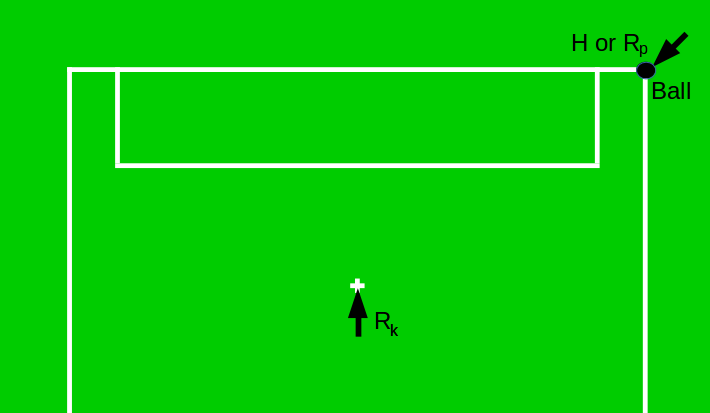
\includegraphics[width=0.8\textwidth]{img/tc_dynamic_kick.png}
\caption{Setup for the moving ball challenge. }
\end{center}
\end{figure}